\documentclass[twoside]{book}

% Packages required by doxygen
\usepackage{fixltx2e}
\usepackage{calc}
\usepackage{doxygen}
\usepackage[export]{adjustbox} % also loads graphicx
\usepackage{graphicx}
\usepackage[utf8]{inputenc}
\usepackage{makeidx}
\usepackage{multicol}
\usepackage{multirow}
\PassOptionsToPackage{warn}{textcomp}
\usepackage{textcomp}
\usepackage[nointegrals]{wasysym}
\usepackage[table]{xcolor}

% Font selection
\usepackage[T1]{fontenc}
\usepackage[scaled=.90]{helvet}
\usepackage{courier}
\usepackage{amssymb}
\usepackage{sectsty}
\renewcommand{\familydefault}{\sfdefault}
\allsectionsfont{%
  \fontseries{bc}\selectfont%
  \color{darkgray}%
}
\renewcommand{\DoxyLabelFont}{%
  \fontseries{bc}\selectfont%
  \color{darkgray}%
}
\newcommand{\+}{\discretionary{\mbox{\scriptsize$\hookleftarrow$}}{}{}}

% Page & text layout
\usepackage{geometry}
\geometry{%
  a4paper,%
  top=2.5cm,%
  bottom=2.5cm,%
  left=2.5cm,%
  right=2.5cm%
}
\tolerance=750
\hfuzz=15pt
\hbadness=750
\setlength{\emergencystretch}{15pt}
\setlength{\parindent}{0cm}
\setlength{\parskip}{3ex plus 2ex minus 2ex}
\makeatletter
\renewcommand{\paragraph}{%
  \@startsection{paragraph}{4}{0ex}{-1.0ex}{1.0ex}{%
    \normalfont\normalsize\bfseries\SS@parafont%
  }%
}
\renewcommand{\subparagraph}{%
  \@startsection{subparagraph}{5}{0ex}{-1.0ex}{1.0ex}{%
    \normalfont\normalsize\bfseries\SS@subparafont%
  }%
}
\makeatother

% Headers & footers
\usepackage{fancyhdr}
\pagestyle{fancyplain}
\fancyhead[LE]{\fancyplain{}{\bfseries\thepage}}
\fancyhead[CE]{\fancyplain{}{}}
\fancyhead[RE]{\fancyplain{}{\bfseries\leftmark}}
\fancyhead[LO]{\fancyplain{}{\bfseries\rightmark}}
\fancyhead[CO]{\fancyplain{}{}}
\fancyhead[RO]{\fancyplain{}{\bfseries\thepage}}
\fancyfoot[LE]{\fancyplain{}{}}
\fancyfoot[CE]{\fancyplain{}{}}
\fancyfoot[RE]{\fancyplain{}{\bfseries\scriptsize Generated by Doxygen }}
\fancyfoot[LO]{\fancyplain{}{\bfseries\scriptsize Generated by Doxygen }}
\fancyfoot[CO]{\fancyplain{}{}}
\fancyfoot[RO]{\fancyplain{}{}}
\renewcommand{\footrulewidth}{0.4pt}
\renewcommand{\chaptermark}[1]{%
  \markboth{#1}{}%
}
\renewcommand{\sectionmark}[1]{%
  \markright{\thesection\ #1}%
}

% Indices & bibliography
\usepackage{natbib}
\usepackage[titles]{tocloft}
\setcounter{tocdepth}{3}
\setcounter{secnumdepth}{5}
\makeindex

% Hyperlinks (required, but should be loaded last)
\usepackage{ifpdf}
\ifpdf
  \usepackage[pdftex,pagebackref=true]{hyperref}
\else
  \usepackage[ps2pdf,pagebackref=true]{hyperref}
\fi
\hypersetup{%
  colorlinks=true,%
  linkcolor=blue,%
  citecolor=blue,%
  unicode%
}

% Custom commands
\newcommand{\clearemptydoublepage}{%
  \newpage{\pagestyle{empty}\cleardoublepage}%
}

\usepackage{caption}
\captionsetup{labelsep=space,justification=centering,font={bf},singlelinecheck=off,skip=4pt,position=top}

%===== C O N T E N T S =====

\begin{document}

% Titlepage & ToC
\hypersetup{pageanchor=false,
             bookmarksnumbered=true,
             pdfencoding=unicode
            }
\pagenumbering{alph}
\begin{titlepage}
\vspace*{7cm}
\begin{center}%
{\Large Project 1 -\/ Voting Application (Team 4) }\\
\vspace*{1cm}
{\large Generated by Doxygen 1.8.13}\\
\end{center}
\end{titlepage}
\clearemptydoublepage
\pagenumbering{roman}
\tableofcontents
\clearemptydoublepage
\pagenumbering{arabic}
\hypersetup{pageanchor=true}

%--- Begin generated contents ---
\chapter{Hierarchical Index}
\section{Class Hierarchy}
This inheritance list is sorted roughly, but not completely, alphabetically\+:\begin{DoxyCompactList}
\item \contentsline{section}{Ballot}{\pageref{classBallot}}{}
\item \contentsline{section}{Candidate}{\pageref{classCandidate}}{}
\item \contentsline{section}{Election}{\pageref{classElection}}{}
\begin{DoxyCompactList}
\item \contentsline{section}{Plurality\+Election}{\pageref{classPluralityElection}}{}
\item \contentsline{section}{S\+T\+V\+Election}{\pageref{classSTVElection}}{}
\end{DoxyCompactList}
\item \contentsline{section}{Voting\+App}{\pageref{classVotingApp}}{}
\end{DoxyCompactList}

\chapter{Class Index}
\section{Class List}
Here are the classes, structs, unions and interfaces with brief descriptions\+:\begin{DoxyCompactList}
\item\contentsline{section}{\hyperlink{classBallot}{Ballot} \\*Necessary functionality to represent a voter\textquotesingle{}s ballot in an election. It is able to represent ballots in both plurality and single-\/tranferrable vote elections. A ballot had an Id, a list of the Candidates in the order they were ranked on the ballot, and a variable indicating the current highest ranked \hyperlink{classCandidate}{Candidate} choice remaining on the ballot }{\pageref{classBallot}}{}
\item\contentsline{section}{\hyperlink{classCandidate}{Candidate} \\*Necessary functionality to represent a candidate in an election. It is able to represent candidates in both plurality and single-\/tranferrable vote elections. A \hyperlink{classCandidate}{Candidate} had an Id, a name, a forward-\/linked list of \hyperlink{classBallot}{Ballot} objects assigned to them, a int representing the count of how many Ballots are assigned to them, double representing the time of when they received their first \hyperlink{classBallot}{Ballot} in an election (needed for S\+TV elections), and boolean indicating whether the \hyperlink{classCandidate}{Candidate} has been declared a winner or a loser yet }{\pageref{classCandidate}}{}
\item\contentsline{section}{\hyperlink{classElection}{Election} \\*Abstract class that provides the necessary functionality to represent an election. While non-\/abstract child classes are required to implement their own \hyperlink{classBallot}{Ballot} tallying algorithms and results, the \hyperlink{classElection}{Election} class provides a template of necessary methods and properties that all types of elections will utilize }{\pageref{classElection}}{}
\item\contentsline{section}{\hyperlink{classPluralityElection}{Plurality\+Election} \\*Child class of the abstract \hyperlink{classElection}{Election} class that provides the necessary functionality to represent a Plurality election }{\pageref{classPluralityElection}}{}
\item\contentsline{section}{\hyperlink{classSTVElection}{S\+T\+V\+Election} \\*Child class of the abstract \hyperlink{classElection}{Election} class that provides the necessary functionality to represent a Single-\/\+Transferrable Vote (ranked choice) election using the Droop algorithm. On top of all of the properties of the \hyperlink{classElection}{Election} class, the \hyperlink{classSTVElection}{S\+T\+V\+Election} class also has a value for the Droop quota, a value indicating whether to turn the \hyperlink{classBallot}{Ballot} shuffle on/off, and a vector that stores the order of the shuffled \hyperlink{classBallot}{Ballot} objects for the election }{\pageref{classSTVElection}}{}
\item\contentsline{section}{\hyperlink{classVotingApp}{Voting\+App} \\*Necessary functionality to run the user interface for the application. It handles all interactions with the user in the interface and initiates the process of running an election after being given all the necessary information by the user. It also provides the necessary functionality to run in a test mode for debugging purposes }{\pageref{classVotingApp}}{}
\end{DoxyCompactList}

\chapter{Class Documentation}
\hypertarget{classBallot}{}\section{Ballot Class Reference}
\label{classBallot}\index{Ballot@{Ballot}}


The \hyperlink{classBallot}{Ballot} class provides the necessary functionality to represent a voter\textquotesingle{}s ballot in an election. It is able to represent ballots in both plurality and single-\/tranferrable vote elections. A ballot had an Id, a list of the Candidates in the order they were ranked on the ballot, and a variable indicating the current highest ranked \hyperlink{classCandidate}{Candidate} choice remaining on the ballot.  




{\ttfamily \#include $<$ballot.\+h$>$}

\subsection*{Public Member Functions}
\begin{DoxyCompactItemize}
\item 
\hyperlink{classBallot_a2155c3611bf5c21502e04845386628cf}{Ballot} (int id, std\+::vector$<$ \hyperlink{classCandidate}{Candidate} $\ast$$>$ choices)
\item 
int \hyperlink{classBallot_a1ff11d3400230f4837fdec904d7e66fd}{get\+Id} ()
\item 
void \hyperlink{classBallot_a1dbe98fb3fc76b2fc4f1a0ee40f3c808}{set\+Id} (int id)
\item 
std\+::vector$<$ \hyperlink{classCandidate}{Candidate} $\ast$ $>$ \hyperlink{classBallot_a7e8730a109ded9c1deeafe75bd1ad55c}{get\+Candidates} ()
\item 
int \hyperlink{classBallot_ae76fc12248878a72a1817adc9fc8361c}{get\+Current\+Choice} ()
\item 
void \hyperlink{classBallot_a1704d1d5b16cc9d3a8e5a2c64c933311}{next\+Choice} ()
\end{DoxyCompactItemize}


\subsection{Detailed Description}
The \hyperlink{classBallot}{Ballot} class provides the necessary functionality to represent a voter\textquotesingle{}s ballot in an election. It is able to represent ballots in both plurality and single-\/tranferrable vote elections. A ballot had an Id, a list of the Candidates in the order they were ranked on the ballot, and a variable indicating the current highest ranked \hyperlink{classCandidate}{Candidate} choice remaining on the ballot. 

\subsection{Constructor \& Destructor Documentation}
\mbox{\Hypertarget{classBallot_a2155c3611bf5c21502e04845386628cf}\label{classBallot_a2155c3611bf5c21502e04845386628cf}} 
\index{Ballot@{Ballot}!Ballot@{Ballot}}
\index{Ballot@{Ballot}!Ballot@{Ballot}}
\subsubsection{\texorpdfstring{Ballot()}{Ballot()}}
{\footnotesize\ttfamily Ballot\+::\+Ballot (\begin{DoxyParamCaption}\item[{int}]{id,  }\item[{std\+::vector$<$ \hyperlink{classCandidate}{Candidate} $\ast$$>$}]{choices }\end{DoxyParamCaption})}

The constructor for the \hyperlink{classBallot}{Ballot} class which sets the initial id of the ballot and the Candidates that were ranked on the \hyperlink{classBallot}{Ballot}. It defaults the current choice index to 0. 
\begin{DoxyParams}{Parameters}
{\em id} & an int that the Id of the \hyperlink{classBallot}{Ballot} object will be set to \\
\hline
{\em choices} & a vector of pointers to Candidates ranked on the \hyperlink{classBallot}{Ballot} object (in order) \\
\hline
\end{DoxyParams}
\begin{DoxyAuthor}{Author}
Brendan Ritchie (ritch167) 
\end{DoxyAuthor}


\subsection{Member Function Documentation}
\mbox{\Hypertarget{classBallot_a7e8730a109ded9c1deeafe75bd1ad55c}\label{classBallot_a7e8730a109ded9c1deeafe75bd1ad55c}} 
\index{Ballot@{Ballot}!get\+Candidates@{get\+Candidates}}
\index{get\+Candidates@{get\+Candidates}!Ballot@{Ballot}}
\subsubsection{\texorpdfstring{get\+Candidates()}{getCandidates()}}
{\footnotesize\ttfamily std\+::vector$<$\hyperlink{classCandidate}{Candidate}$\ast$$>$ Ballot\+::get\+Candidates (\begin{DoxyParamCaption}{ }\end{DoxyParamCaption})}

This method returns the vector of pointers to Candidates ranked on the \hyperlink{classBallot}{Ballot} object (in order) \begin{DoxyAuthor}{Author}
Brendan Ritchie (ritch167) 
\end{DoxyAuthor}
\mbox{\Hypertarget{classBallot_ae76fc12248878a72a1817adc9fc8361c}\label{classBallot_ae76fc12248878a72a1817adc9fc8361c}} 
\index{Ballot@{Ballot}!get\+Current\+Choice@{get\+Current\+Choice}}
\index{get\+Current\+Choice@{get\+Current\+Choice}!Ballot@{Ballot}}
\subsubsection{\texorpdfstring{get\+Current\+Choice()}{getCurrentChoice()}}
{\footnotesize\ttfamily int Ballot\+::get\+Current\+Choice (\begin{DoxyParamCaption}{ }\end{DoxyParamCaption})}

This method returns the index of the current highest ranked \hyperlink{classCandidate}{Candidate} choice in the vector of Candidates ranked on the \hyperlink{classBallot}{Ballot} object \begin{DoxyAuthor}{Author}
Brendan Ritchie (ritch167) 
\end{DoxyAuthor}
\mbox{\Hypertarget{classBallot_a1ff11d3400230f4837fdec904d7e66fd}\label{classBallot_a1ff11d3400230f4837fdec904d7e66fd}} 
\index{Ballot@{Ballot}!get\+Id@{get\+Id}}
\index{get\+Id@{get\+Id}!Ballot@{Ballot}}
\subsubsection{\texorpdfstring{get\+Id()}{getId()}}
{\footnotesize\ttfamily int Ballot\+::get\+Id (\begin{DoxyParamCaption}{ }\end{DoxyParamCaption})}

This method returns the Id of the \hyperlink{classBallot}{Ballot} object \begin{DoxyAuthor}{Author}
Brendan Ritchie (ritch167) 
\end{DoxyAuthor}
\mbox{\Hypertarget{classBallot_a1704d1d5b16cc9d3a8e5a2c64c933311}\label{classBallot_a1704d1d5b16cc9d3a8e5a2c64c933311}} 
\index{Ballot@{Ballot}!next\+Choice@{next\+Choice}}
\index{next\+Choice@{next\+Choice}!Ballot@{Ballot}}
\subsubsection{\texorpdfstring{next\+Choice()}{nextChoice()}}
{\footnotesize\ttfamily void Ballot\+::next\+Choice (\begin{DoxyParamCaption}{ }\end{DoxyParamCaption})}

This method sets the current\+Choice to the next \hyperlink{classCandidate}{Candidate} in order \begin{DoxyAuthor}{Author}
Yiwen Xu (xu000515) 
\end{DoxyAuthor}
\mbox{\Hypertarget{classBallot_a1dbe98fb3fc76b2fc4f1a0ee40f3c808}\label{classBallot_a1dbe98fb3fc76b2fc4f1a0ee40f3c808}} 
\index{Ballot@{Ballot}!set\+Id@{set\+Id}}
\index{set\+Id@{set\+Id}!Ballot@{Ballot}}
\subsubsection{\texorpdfstring{set\+Id()}{setId()}}
{\footnotesize\ttfamily void Ballot\+::set\+Id (\begin{DoxyParamCaption}\item[{int}]{id }\end{DoxyParamCaption})}

This method sets the Id of the \hyperlink{classBallot}{Ballot} object 
\begin{DoxyParams}{Parameters}
{\em id} & an int that the Id of the \hyperlink{classBallot}{Ballot} object will be set to \\
\hline
\end{DoxyParams}
\begin{DoxyAuthor}{Author}
Brendan Ritchie (ritch167) 
\end{DoxyAuthor}


The documentation for this class was generated from the following file\+:\begin{DoxyCompactItemize}
\item 
/home/ritch167/csci5801/repo-\/\+Team4/\+Project2/src/ballot.\+h\end{DoxyCompactItemize}

\hypertarget{classCandidate}{}\section{Candidate Class Reference}
\label{classCandidate}\index{Candidate@{Candidate}}


The \hyperlink{classCandidate}{Candidate} class provides the necessary functionality to represent a candidate in an election. It is able to represent candidates in both plurality and single-\/tranferrable vote elections. A \hyperlink{classCandidate}{Candidate} had an Id, a name, a forward-\/linked list of \hyperlink{classBallot}{Ballot} objects assigned to them, a int representing the count of how many Ballots are assigned to them, double representing the time of when they received their first \hyperlink{classBallot}{Ballot} in an election (needed for S\+TV elections), and boolean indicating whether the \hyperlink{classCandidate}{Candidate} has been declared a winner or a loser yet.  




{\ttfamily \#include $<$candidate.\+h$>$}

\subsection*{Public Member Functions}
\begin{DoxyCompactItemize}
\item 
\hyperlink{classCandidate_a58b3815b3b93c161c47165e3725b704a}{Candidate} (int id, std\+::string name)
\item 
int \hyperlink{classCandidate_a50e7cd31dc68665860932987ad2ffea6}{get\+Id} ()
\item 
std\+::string \hyperlink{classCandidate_af862d92e21d66d74f1d5cae92937d3da}{get\+Name} ()
\item 
std\+::list$<$ \hyperlink{classBallot}{Ballot} $\ast$ $>$ \hyperlink{classCandidate_a2bd33d32107aa062ef8bd82e8b2ee7e9}{get\+Ballots\+For} ()
\item 
void \hyperlink{classCandidate_abbe882aa5bad2f1b769c3df933495703}{add\+Ballot} (\hyperlink{classBallot}{Ballot} $\ast$new\+\_\+ballot)
\item 
\hyperlink{classBallot}{Ballot} $\ast$ \hyperlink{classCandidate_a329eae2002b3584594dd10c92b5f6f51}{remove\+Ballot} ()
\item 
int \hyperlink{classCandidate_abe5eb062e31ef3602b4434e5e9f1e596}{get\+Ballots\+For\+Size} ()
\item 
double \hyperlink{classCandidate_acb99e3ce6e39413c36b1181f67b870ff}{get\+When\+Got\+First\+Ballot} ()
\item 
void \hyperlink{classCandidate_a97be1d696ea97201ec69a75bf708d9f2}{set\+When\+Got\+First\+Ballot} (double time)
\item 
bool \hyperlink{classCandidate_ac00fcb7914f89cca8bb02ed2e6d6f4e4}{get\+Assigned\+Status} ()
\item 
void \hyperlink{classCandidate_a9b407c109b00124423fbe4a722a503c2}{set\+Assigned\+Status} (bool status)
\end{DoxyCompactItemize}


\subsection{Detailed Description}
The \hyperlink{classCandidate}{Candidate} class provides the necessary functionality to represent a candidate in an election. It is able to represent candidates in both plurality and single-\/tranferrable vote elections. A \hyperlink{classCandidate}{Candidate} had an Id, a name, a forward-\/linked list of \hyperlink{classBallot}{Ballot} objects assigned to them, a int representing the count of how many Ballots are assigned to them, double representing the time of when they received their first \hyperlink{classBallot}{Ballot} in an election (needed for S\+TV elections), and boolean indicating whether the \hyperlink{classCandidate}{Candidate} has been declared a winner or a loser yet. 

\subsection{Constructor \& Destructor Documentation}
\mbox{\Hypertarget{classCandidate_a58b3815b3b93c161c47165e3725b704a}\label{classCandidate_a58b3815b3b93c161c47165e3725b704a}} 
\index{Candidate@{Candidate}!Candidate@{Candidate}}
\index{Candidate@{Candidate}!Candidate@{Candidate}}
\subsubsection{\texorpdfstring{Candidate()}{Candidate()}}
{\footnotesize\ttfamily Candidate\+::\+Candidate (\begin{DoxyParamCaption}\item[{int}]{id,  }\item[{std\+::string}]{name }\end{DoxyParamCaption})}

The constructor for the \hyperlink{classCandidate}{Candidate} class sets the initial id of the ballot and the \hyperlink{classCandidate}{Candidate} object\textquotesingle{}s name. It defaults the count of its \hyperlink{classBallot}{Ballot} objects for to 0, when they got their first ballot to -\/1.\+0, and their winner/loser assigned status to false. 
\begin{DoxyParams}{Parameters}
{\em id} & an int that the Id of the \hyperlink{classCandidate}{Candidate} object will be set to \\
\hline
{\em name} & a string that the name of the \hyperlink{classCandidate}{Candidate} will be set to \\
\hline
\end{DoxyParams}
\begin{DoxyAuthor}{Author}
Brendan Ritchie (ritch167) 
\end{DoxyAuthor}


\subsection{Member Function Documentation}
\mbox{\Hypertarget{classCandidate_abbe882aa5bad2f1b769c3df933495703}\label{classCandidate_abbe882aa5bad2f1b769c3df933495703}} 
\index{Candidate@{Candidate}!add\+Ballot@{add\+Ballot}}
\index{add\+Ballot@{add\+Ballot}!Candidate@{Candidate}}
\subsubsection{\texorpdfstring{add\+Ballot()}{addBallot()}}
{\footnotesize\ttfamily void Candidate\+::add\+Ballot (\begin{DoxyParamCaption}\item[{\hyperlink{classBallot}{Ballot} $\ast$}]{new\+\_\+ballot }\end{DoxyParamCaption})}

This method is responsible for adding new \hyperlink{classBallot}{Ballot} to the end of the list ballots\+For of the \hyperlink{classCandidate}{Candidate}. 
\begin{DoxyParams}{Parameters}
{\em new\+\_\+ballot} & a pointer to the new \hyperlink{classBallot}{Ballot} which will be added to the list \\
\hline
\end{DoxyParams}
\begin{DoxyAuthor}{Author}
Yiwen Xu (xu000515) 
\end{DoxyAuthor}
\mbox{\Hypertarget{classCandidate_ac00fcb7914f89cca8bb02ed2e6d6f4e4}\label{classCandidate_ac00fcb7914f89cca8bb02ed2e6d6f4e4}} 
\index{Candidate@{Candidate}!get\+Assigned\+Status@{get\+Assigned\+Status}}
\index{get\+Assigned\+Status@{get\+Assigned\+Status}!Candidate@{Candidate}}
\subsubsection{\texorpdfstring{get\+Assigned\+Status()}{getAssignedStatus()}}
{\footnotesize\ttfamily bool Candidate\+::get\+Assigned\+Status (\begin{DoxyParamCaption}{ }\end{DoxyParamCaption})}

This method returns the boolean indicating whether the \hyperlink{classCandidate}{Candidate} object has been declared a winner or a loser yet. \begin{DoxyAuthor}{Author}
Brendan Ritchie (ritch167) 
\end{DoxyAuthor}
\mbox{\Hypertarget{classCandidate_a2bd33d32107aa062ef8bd82e8b2ee7e9}\label{classCandidate_a2bd33d32107aa062ef8bd82e8b2ee7e9}} 
\index{Candidate@{Candidate}!get\+Ballots\+For@{get\+Ballots\+For}}
\index{get\+Ballots\+For@{get\+Ballots\+For}!Candidate@{Candidate}}
\subsubsection{\texorpdfstring{get\+Ballots\+For()}{getBallotsFor()}}
{\footnotesize\ttfamily std\+::list$<$\hyperlink{classBallot}{Ballot} $\ast$$>$ Candidate\+::get\+Ballots\+For (\begin{DoxyParamCaption}{ }\end{DoxyParamCaption})}

This method returns the list of pointers to \hyperlink{classBallot}{Ballot} objects assigned to the \hyperlink{classCandidate}{Candidate} object. \begin{DoxyAuthor}{Author}
Brendan Ritchie (ritch167) 
\end{DoxyAuthor}
\mbox{\Hypertarget{classCandidate_abe5eb062e31ef3602b4434e5e9f1e596}\label{classCandidate_abe5eb062e31ef3602b4434e5e9f1e596}} 
\index{Candidate@{Candidate}!get\+Ballots\+For\+Size@{get\+Ballots\+For\+Size}}
\index{get\+Ballots\+For\+Size@{get\+Ballots\+For\+Size}!Candidate@{Candidate}}
\subsubsection{\texorpdfstring{get\+Ballots\+For\+Size()}{getBallotsForSize()}}
{\footnotesize\ttfamily int Candidate\+::get\+Ballots\+For\+Size (\begin{DoxyParamCaption}{ }\end{DoxyParamCaption})}

This method returns the the count of how many Ballots objects are assigned to the \hyperlink{classCandidate}{Candidate} objects. \begin{DoxyAuthor}{Author}
Brendan Ritchie (ritch167) 
\end{DoxyAuthor}
\mbox{\Hypertarget{classCandidate_a50e7cd31dc68665860932987ad2ffea6}\label{classCandidate_a50e7cd31dc68665860932987ad2ffea6}} 
\index{Candidate@{Candidate}!get\+Id@{get\+Id}}
\index{get\+Id@{get\+Id}!Candidate@{Candidate}}
\subsubsection{\texorpdfstring{get\+Id()}{getId()}}
{\footnotesize\ttfamily int Candidate\+::get\+Id (\begin{DoxyParamCaption}{ }\end{DoxyParamCaption})}

This method returns the Id of the \hyperlink{classCandidate}{Candidate} object. \begin{DoxyAuthor}{Author}
Brendan Ritchie (ritch167) 
\end{DoxyAuthor}
\mbox{\Hypertarget{classCandidate_af862d92e21d66d74f1d5cae92937d3da}\label{classCandidate_af862d92e21d66d74f1d5cae92937d3da}} 
\index{Candidate@{Candidate}!get\+Name@{get\+Name}}
\index{get\+Name@{get\+Name}!Candidate@{Candidate}}
\subsubsection{\texorpdfstring{get\+Name()}{getName()}}
{\footnotesize\ttfamily std\+::string Candidate\+::get\+Name (\begin{DoxyParamCaption}{ }\end{DoxyParamCaption})}

This method returns the name of the \hyperlink{classCandidate}{Candidate} object. \begin{DoxyAuthor}{Author}
Brendan Ritchie (ritch167) 
\end{DoxyAuthor}
\mbox{\Hypertarget{classCandidate_acb99e3ce6e39413c36b1181f67b870ff}\label{classCandidate_acb99e3ce6e39413c36b1181f67b870ff}} 
\index{Candidate@{Candidate}!get\+When\+Got\+First\+Ballot@{get\+When\+Got\+First\+Ballot}}
\index{get\+When\+Got\+First\+Ballot@{get\+When\+Got\+First\+Ballot}!Candidate@{Candidate}}
\subsubsection{\texorpdfstring{get\+When\+Got\+First\+Ballot()}{getWhenGotFirstBallot()}}
{\footnotesize\ttfamily double Candidate\+::get\+When\+Got\+First\+Ballot (\begin{DoxyParamCaption}{ }\end{DoxyParamCaption})}

This method returns the double representing the time of when the \hyperlink{classCandidate}{Candidate} object received their first \hyperlink{classBallot}{Ballot} in an election (needed for S\+TV elections). \begin{DoxyAuthor}{Author}
Brendan Ritchie (ritch167) 
\end{DoxyAuthor}
\mbox{\Hypertarget{classCandidate_a329eae2002b3584594dd10c92b5f6f51}\label{classCandidate_a329eae2002b3584594dd10c92b5f6f51}} 
\index{Candidate@{Candidate}!remove\+Ballot@{remove\+Ballot}}
\index{remove\+Ballot@{remove\+Ballot}!Candidate@{Candidate}}
\subsubsection{\texorpdfstring{remove\+Ballot()}{removeBallot()}}
{\footnotesize\ttfamily \hyperlink{classBallot}{Ballot}$\ast$ Candidate\+::remove\+Ballot (\begin{DoxyParamCaption}{ }\end{DoxyParamCaption})}

This method removes a \hyperlink{classBallot}{Ballot} from the front of the list ballots\+For for the \hyperlink{classCandidate}{Candidate} and returns that \hyperlink{classBallot}{Ballot}. \begin{DoxyAuthor}{Author}
Yiwen Xu (xu000515) 
\end{DoxyAuthor}
\mbox{\Hypertarget{classCandidate_a9b407c109b00124423fbe4a722a503c2}\label{classCandidate_a9b407c109b00124423fbe4a722a503c2}} 
\index{Candidate@{Candidate}!set\+Assigned\+Status@{set\+Assigned\+Status}}
\index{set\+Assigned\+Status@{set\+Assigned\+Status}!Candidate@{Candidate}}
\subsubsection{\texorpdfstring{set\+Assigned\+Status()}{setAssignedStatus()}}
{\footnotesize\ttfamily void Candidate\+::set\+Assigned\+Status (\begin{DoxyParamCaption}\item[{bool}]{status }\end{DoxyParamCaption})}

This method sets the status indicating whether the \hyperlink{classCandidate}{Candidate} object has been declared a winner or a loser yet. 
\begin{DoxyParams}{Parameters}
{\em status} & a boolean indicating whether the \hyperlink{classCandidate}{Candidate} has been assigned or not \\
\hline
\end{DoxyParams}
\begin{DoxyAuthor}{Author}
Brendan Ritchie (ritch167) 
\end{DoxyAuthor}
\mbox{\Hypertarget{classCandidate_a97be1d696ea97201ec69a75bf708d9f2}\label{classCandidate_a97be1d696ea97201ec69a75bf708d9f2}} 
\index{Candidate@{Candidate}!set\+When\+Got\+First\+Ballot@{set\+When\+Got\+First\+Ballot}}
\index{set\+When\+Got\+First\+Ballot@{set\+When\+Got\+First\+Ballot}!Candidate@{Candidate}}
\subsubsection{\texorpdfstring{set\+When\+Got\+First\+Ballot()}{setWhenGotFirstBallot()}}
{\footnotesize\ttfamily void Candidate\+::set\+When\+Got\+First\+Ballot (\begin{DoxyParamCaption}\item[{double}]{time }\end{DoxyParamCaption})}

This method sets the time when the \hyperlink{classCandidate}{Candidate} object received their first \hyperlink{classBallot}{Ballot} in an election (needed for S\+TV elections). 
\begin{DoxyParams}{Parameters}
{\em time} & an double representing the number of seconds since the election algorithm started processing \\
\hline
\end{DoxyParams}
\begin{DoxyAuthor}{Author}
Brendan Ritchie (ritch167) 
\end{DoxyAuthor}


The documentation for this class was generated from the following file\+:\begin{DoxyCompactItemize}
\item 
/home/ritch167/csci5801/repo-\/\+Team4/\+Project1/src/candidate.\+h\end{DoxyCompactItemize}

\hypertarget{classElection}{}\section{Election Class Reference}
\label{classElection}\index{Election@{Election}}


The \hyperlink{classElection}{Election} class is an abstract class that provides the necessary functionality to represent an election. While non-\/abstract child classes are required to implement their own \hyperlink{classBallot}{Ballot} tallying algorithms and results, the \hyperlink{classElection}{Election} class provides a template of necessary methods and properties that all types of elections will utilize.  




{\ttfamily \#include $<$election.\+h$>$}



Inheritance diagram for Election\+:\nopagebreak
\begin{figure}[H]
\begin{center}
\leavevmode
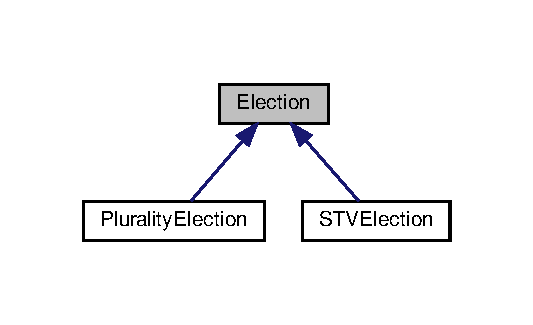
\includegraphics[width=256pt]{classElection__inherit__graph}
\end{center}
\end{figure}
\subsection*{Public Member Functions}
\begin{DoxyCompactItemize}
\item 
\hyperlink{classElection_a4f6dd551dbe4276f97b565ce2fd8fb5d}{Election} (std\+::string type, int seats, std\+::vector$<$ \hyperlink{classCandidate}{Candidate} $\ast$$>$ cands, std\+::vector$<$ \hyperlink{classBallot}{Ballot} $\ast$$>$ bals)
\item 
std\+::string \hyperlink{classElection_ae49e7f5d36d4afc23ed81b4df4ae658c}{get\+Type} ()
\item 
int \hyperlink{classElection_a0b68106ee52f33286364ef5d617d77ee}{get\+Num\+Seats} ()
\item 
std\+::vector$<$ \hyperlink{classCandidate}{Candidate} $\ast$ $>$ \hyperlink{classElection_a1514ca134f88464b026cc51da5076d29}{get\+Candidates} ()
\item 
std\+::vector$<$ \hyperlink{classBallot}{Ballot} $\ast$ $>$ \hyperlink{classElection_abd0c0a7649a3f5d87541e3f65fec7244}{get\+Ballots} ()
\item 
std\+::vector$<$ \hyperlink{classCandidate}{Candidate} $\ast$ $>$ \hyperlink{classElection_a8cc211952aa00399649c8660eb62189c}{get\+Winners} ()
\item 
std\+::vector$<$ \hyperlink{classCandidate}{Candidate} $\ast$ $>$ \hyperlink{classElection_a34dfd0c1c6519073d38e85790c839f8b}{get\+Losers} ()
\item 
std\+::string \hyperlink{classElection_ae55fafa9a82cca3c20b2343fed3f7250}{get\+Audit\+File\+Path} ()
\item 
virtual void \hyperlink{classElection_a059659576ebb0416ecd8005f684461d6}{run\+Algorithm} ()=0
\item 
virtual std\+::string \hyperlink{classElection_a6a6f4f301db86628b8d962281a19bf74}{get\+Results} ()=0
\end{DoxyCompactItemize}
\subsection*{Protected Member Functions}
\begin{DoxyCompactItemize}
\item 
void \hyperlink{classElection_ad50f3b2f39c7e7ee96f1987c9dddb926}{set\+Audit\+File\+Path} (std\+::string name)
\item 
void \hyperlink{classElection_abd52b6c894a9f2a0a0a104e9f290f9a7}{write\+To\+Audit\+File} ()
\item 
void \hyperlink{classElection_a6b6bac6b3c0789a311f1daf8e9d4a31c}{add\+Winner} (\hyperlink{classCandidate}{Candidate} $\ast$win)
\item 
void \hyperlink{classElection_a732076e36548e51e8c675598ac4a03dd}{add\+Loser} (\hyperlink{classCandidate}{Candidate} $\ast$lose)
\end{DoxyCompactItemize}
\subsection*{Protected Attributes}
\begin{DoxyCompactItemize}
\item 
\mbox{\Hypertarget{classElection_a50e140cb8138c91be243bec30a78125e}\label{classElection_a50e140cb8138c91be243bec30a78125e}} 
std\+::string {\bfseries type\+\_\+}
\item 
\mbox{\Hypertarget{classElection_a9c116f9c551c84348c026ab9a05ab0f4}\label{classElection_a9c116f9c551c84348c026ab9a05ab0f4}} 
int {\bfseries num\+Seats\+\_\+}
\item 
\mbox{\Hypertarget{classElection_aebd1b5662e37beaac28acae18fda15f6}\label{classElection_aebd1b5662e37beaac28acae18fda15f6}} 
std\+::vector$<$ \hyperlink{classCandidate}{Candidate} $\ast$ $>$ {\bfseries candidates\+\_\+}
\item 
\mbox{\Hypertarget{classElection_a309d7e1f884da5b37c9c582f8ffc559c}\label{classElection_a309d7e1f884da5b37c9c582f8ffc559c}} 
std\+::vector$<$ \hyperlink{classBallot}{Ballot} $\ast$ $>$ {\bfseries ballots\+\_\+}
\item 
\mbox{\Hypertarget{classElection_a13d2d174fb9a3b3044f078e8560c226a}\label{classElection_a13d2d174fb9a3b3044f078e8560c226a}} 
std\+::vector$<$ \hyperlink{classCandidate}{Candidate} $\ast$ $>$ {\bfseries winners\+\_\+}
\item 
\mbox{\Hypertarget{classElection_ac8e2a461ac014f2c45d1de8ca4d940ec}\label{classElection_ac8e2a461ac014f2c45d1de8ca4d940ec}} 
std\+::vector$<$ \hyperlink{classCandidate}{Candidate} $\ast$ $>$ {\bfseries losers\+\_\+}
\item 
\mbox{\Hypertarget{classElection_ad564bb183a5a0679398d0a74c213a92a}\label{classElection_ad564bb183a5a0679398d0a74c213a92a}} 
std\+::string {\bfseries audit\+File\+Path\+\_\+}
\item 
\mbox{\Hypertarget{classElection_a5dcc64f43ede2f4878fbe15db51b2c4c}\label{classElection_a5dcc64f43ede2f4878fbe15db51b2c4c}} 
std\+::stringstream {\bfseries audit\+Text\+\_\+}
\end{DoxyCompactItemize}


\subsection{Detailed Description}
The \hyperlink{classElection}{Election} class is an abstract class that provides the necessary functionality to represent an election. While non-\/abstract child classes are required to implement their own \hyperlink{classBallot}{Ballot} tallying algorithms and results, the \hyperlink{classElection}{Election} class provides a template of necessary methods and properties that all types of elections will utilize. 

\subsection{Constructor \& Destructor Documentation}
\mbox{\Hypertarget{classElection_a4f6dd551dbe4276f97b565ce2fd8fb5d}\label{classElection_a4f6dd551dbe4276f97b565ce2fd8fb5d}} 
\index{Election@{Election}!Election@{Election}}
\index{Election@{Election}!Election@{Election}}
\subsubsection{\texorpdfstring{Election()}{Election()}}
{\footnotesize\ttfamily Election\+::\+Election (\begin{DoxyParamCaption}\item[{std\+::string}]{type,  }\item[{int}]{seats,  }\item[{std\+::vector$<$ \hyperlink{classCandidate}{Candidate} $\ast$$>$}]{cands,  }\item[{std\+::vector$<$ \hyperlink{classBallot}{Ballot} $\ast$$>$}]{bals }\end{DoxyParamCaption})}

The constructor for the \hyperlink{classElection}{Election} class sets the type of the election, the number of seats in the election, the vector that stores the Candidates who are running in the election, and the vector that stores the Ballots cast in the election. It also defaults the name of the audit file path to the empty string. 
\begin{DoxyParams}{Parameters}
{\em type} & a string that indicates the election type \\
\hline
{\em seats} & an int that indicates the number of seats in the election \\
\hline
{\em cands} & a vector of Candidates who are up for election \\
\hline
{\em bals} & a vector of Ballots that were cast in the election \\
\hline
\end{DoxyParams}
\begin{DoxyAuthor}{Author}
Brendan Ritchie (ritch167) 
\end{DoxyAuthor}


\subsection{Member Function Documentation}
\mbox{\Hypertarget{classElection_a732076e36548e51e8c675598ac4a03dd}\label{classElection_a732076e36548e51e8c675598ac4a03dd}} 
\index{Election@{Election}!add\+Loser@{add\+Loser}}
\index{add\+Loser@{add\+Loser}!Election@{Election}}
\subsubsection{\texorpdfstring{add\+Loser()}{addLoser()}}
{\footnotesize\ttfamily void Election\+::add\+Loser (\begin{DoxyParamCaption}\item[{\hyperlink{classCandidate}{Candidate} $\ast$}]{lose }\end{DoxyParamCaption})\hspace{0.3cm}{\ttfamily [protected]}}

This methods adds a candidate to losers\+\_\+ vector which is a vector of Candidates. \begin{DoxyAuthor}{Author}
Yifan Zhang(zhan4372) 
\end{DoxyAuthor}
\mbox{\Hypertarget{classElection_a6b6bac6b3c0789a311f1daf8e9d4a31c}\label{classElection_a6b6bac6b3c0789a311f1daf8e9d4a31c}} 
\index{Election@{Election}!add\+Winner@{add\+Winner}}
\index{add\+Winner@{add\+Winner}!Election@{Election}}
\subsubsection{\texorpdfstring{add\+Winner()}{addWinner()}}
{\footnotesize\ttfamily void Election\+::add\+Winner (\begin{DoxyParamCaption}\item[{\hyperlink{classCandidate}{Candidate} $\ast$}]{win }\end{DoxyParamCaption})\hspace{0.3cm}{\ttfamily [protected]}}

This methods adds a candidate to winners\+\_\+ vector which is a vector of Candidates. \begin{DoxyAuthor}{Author}
Yifan Zhang(zhan4372) 
\end{DoxyAuthor}
\mbox{\Hypertarget{classElection_ae55fafa9a82cca3c20b2343fed3f7250}\label{classElection_ae55fafa9a82cca3c20b2343fed3f7250}} 
\index{Election@{Election}!get\+Audit\+File\+Path@{get\+Audit\+File\+Path}}
\index{get\+Audit\+File\+Path@{get\+Audit\+File\+Path}!Election@{Election}}
\subsubsection{\texorpdfstring{get\+Audit\+File\+Path()}{getAuditFilePath()}}
{\footnotesize\ttfamily std\+::string Election\+::get\+Audit\+File\+Path (\begin{DoxyParamCaption}{ }\end{DoxyParamCaption})}

This method returns the path for the audit file in the \hyperlink{classElection}{Election} object. \begin{DoxyAuthor}{Author}
Brendan Ritchie (ritch167) 
\end{DoxyAuthor}
\mbox{\Hypertarget{classElection_abd0c0a7649a3f5d87541e3f65fec7244}\label{classElection_abd0c0a7649a3f5d87541e3f65fec7244}} 
\index{Election@{Election}!get\+Ballots@{get\+Ballots}}
\index{get\+Ballots@{get\+Ballots}!Election@{Election}}
\subsubsection{\texorpdfstring{get\+Ballots()}{getBallots()}}
{\footnotesize\ttfamily std\+::vector$<$\hyperlink{classBallot}{Ballot}$\ast$$>$ Election\+::get\+Ballots (\begin{DoxyParamCaption}{ }\end{DoxyParamCaption})}

This method returns the vector of \hyperlink{classBallot}{Ballot} pointers in the \hyperlink{classElection}{Election} object. \begin{DoxyAuthor}{Author}
Brendan Ritchie (ritch167) 
\end{DoxyAuthor}
\mbox{\Hypertarget{classElection_a1514ca134f88464b026cc51da5076d29}\label{classElection_a1514ca134f88464b026cc51da5076d29}} 
\index{Election@{Election}!get\+Candidates@{get\+Candidates}}
\index{get\+Candidates@{get\+Candidates}!Election@{Election}}
\subsubsection{\texorpdfstring{get\+Candidates()}{getCandidates()}}
{\footnotesize\ttfamily std\+::vector$<$\hyperlink{classCandidate}{Candidate}$\ast$$>$ Election\+::get\+Candidates (\begin{DoxyParamCaption}{ }\end{DoxyParamCaption})}

This method returns the vector of \hyperlink{classCandidate}{Candidate} pointers in the \hyperlink{classElection}{Election} object. \begin{DoxyAuthor}{Author}
Brendan Ritchie (ritch167) 
\end{DoxyAuthor}
\mbox{\Hypertarget{classElection_a34dfd0c1c6519073d38e85790c839f8b}\label{classElection_a34dfd0c1c6519073d38e85790c839f8b}} 
\index{Election@{Election}!get\+Losers@{get\+Losers}}
\index{get\+Losers@{get\+Losers}!Election@{Election}}
\subsubsection{\texorpdfstring{get\+Losers()}{getLosers()}}
{\footnotesize\ttfamily std\+::vector$<$\hyperlink{classCandidate}{Candidate}$\ast$$>$ Election\+::get\+Losers (\begin{DoxyParamCaption}{ }\end{DoxyParamCaption})}

This method returns the losers which is a vector of \hyperlink{classCandidate}{Candidate} pointers in the \hyperlink{classElection}{Election} object. \begin{DoxyAuthor}{Author}
Brendan Ritchie (ritch167) 
\end{DoxyAuthor}
\mbox{\Hypertarget{classElection_a0b68106ee52f33286364ef5d617d77ee}\label{classElection_a0b68106ee52f33286364ef5d617d77ee}} 
\index{Election@{Election}!get\+Num\+Seats@{get\+Num\+Seats}}
\index{get\+Num\+Seats@{get\+Num\+Seats}!Election@{Election}}
\subsubsection{\texorpdfstring{get\+Num\+Seats()}{getNumSeats()}}
{\footnotesize\ttfamily int Election\+::get\+Num\+Seats (\begin{DoxyParamCaption}{ }\end{DoxyParamCaption})}

This method returns the number of the seats of the \hyperlink{classElection}{Election} object. \begin{DoxyAuthor}{Author}
Brendan Ritchie (ritch167) 
\end{DoxyAuthor}
\mbox{\Hypertarget{classElection_a6a6f4f301db86628b8d962281a19bf74}\label{classElection_a6a6f4f301db86628b8d962281a19bf74}} 
\index{Election@{Election}!get\+Results@{get\+Results}}
\index{get\+Results@{get\+Results}!Election@{Election}}
\subsubsection{\texorpdfstring{get\+Results()}{getResults()}}
{\footnotesize\ttfamily virtual std\+::string Election\+::get\+Results (\begin{DoxyParamCaption}{ }\end{DoxyParamCaption})\hspace{0.3cm}{\ttfamily [pure virtual]}}

This pure virtual method will be implemented in the child classes of \hyperlink{classElection}{Election} and will be responsible for compiling the results for the specific election type 

Implemented in \hyperlink{classSTVElection_ae7efa73091c87add327d71ff5f943c3c}{S\+T\+V\+Election}, and \hyperlink{classPluralityElection_a60f88a34588ca87678b0f5367adf1a55}{Plurality\+Election}.

\mbox{\Hypertarget{classElection_ae49e7f5d36d4afc23ed81b4df4ae658c}\label{classElection_ae49e7f5d36d4afc23ed81b4df4ae658c}} 
\index{Election@{Election}!get\+Type@{get\+Type}}
\index{get\+Type@{get\+Type}!Election@{Election}}
\subsubsection{\texorpdfstring{get\+Type()}{getType()}}
{\footnotesize\ttfamily std\+::string Election\+::get\+Type (\begin{DoxyParamCaption}{ }\end{DoxyParamCaption})}

This method returns the type of the \hyperlink{classElection}{Election} object. \begin{DoxyAuthor}{Author}
Brendan Ritchie (ritch167) 
\end{DoxyAuthor}
\mbox{\Hypertarget{classElection_a8cc211952aa00399649c8660eb62189c}\label{classElection_a8cc211952aa00399649c8660eb62189c}} 
\index{Election@{Election}!get\+Winners@{get\+Winners}}
\index{get\+Winners@{get\+Winners}!Election@{Election}}
\subsubsection{\texorpdfstring{get\+Winners()}{getWinners()}}
{\footnotesize\ttfamily std\+::vector$<$\hyperlink{classCandidate}{Candidate}$\ast$$>$ Election\+::get\+Winners (\begin{DoxyParamCaption}{ }\end{DoxyParamCaption})}

This method returns the winners which is a vector of \hyperlink{classCandidate}{Candidate} pointers in the \hyperlink{classElection}{Election} object. \begin{DoxyAuthor}{Author}
Brendan Ritchie (ritch167) 
\end{DoxyAuthor}
\mbox{\Hypertarget{classElection_a059659576ebb0416ecd8005f684461d6}\label{classElection_a059659576ebb0416ecd8005f684461d6}} 
\index{Election@{Election}!run\+Algorithm@{run\+Algorithm}}
\index{run\+Algorithm@{run\+Algorithm}!Election@{Election}}
\subsubsection{\texorpdfstring{run\+Algorithm()}{runAlgorithm()}}
{\footnotesize\ttfamily virtual void Election\+::run\+Algorithm (\begin{DoxyParamCaption}{ }\end{DoxyParamCaption})\hspace{0.3cm}{\ttfamily [pure virtual]}}

This pure virtual method will be implemented in the child classes of \hyperlink{classElection}{Election} and will be responsible for running the speicific election type\textquotesingle{}s vote tallying algorithm. 

Implemented in \hyperlink{classSTVElection_ac4e0339e3cb97add1a22c9af7233df17}{S\+T\+V\+Election}, and \hyperlink{classPluralityElection_a9517806e8ba40496c49013acc7ad9ca5}{Plurality\+Election}.

\mbox{\Hypertarget{classElection_ad50f3b2f39c7e7ee96f1987c9dddb926}\label{classElection_ad50f3b2f39c7e7ee96f1987c9dddb926}} 
\index{Election@{Election}!set\+Audit\+File\+Path@{set\+Audit\+File\+Path}}
\index{set\+Audit\+File\+Path@{set\+Audit\+File\+Path}!Election@{Election}}
\subsubsection{\texorpdfstring{set\+Audit\+File\+Path()}{setAuditFilePath()}}
{\footnotesize\ttfamily void Election\+::set\+Audit\+File\+Path (\begin{DoxyParamCaption}\item[{std\+::string}]{name }\end{DoxyParamCaption})\hspace{0.3cm}{\ttfamily [protected]}}

This method sets the audit\+File\+Path of the \hyperlink{classElection}{Election} object 
\begin{DoxyParams}{Parameters}
{\em name} & a string that the audit\+File\+Path of the \hyperlink{classElection}{Election} object will be set to \\
\hline
\end{DoxyParams}
\begin{DoxyAuthor}{Author}
Brendan Ritchie (ritch167) 
\end{DoxyAuthor}
\mbox{\Hypertarget{classElection_abd52b6c894a9f2a0a0a104e9f290f9a7}\label{classElection_abd52b6c894a9f2a0a0a104e9f290f9a7}} 
\index{Election@{Election}!write\+To\+Audit\+File@{write\+To\+Audit\+File}}
\index{write\+To\+Audit\+File@{write\+To\+Audit\+File}!Election@{Election}}
\subsubsection{\texorpdfstring{write\+To\+Audit\+File()}{writeToAuditFile()}}
{\footnotesize\ttfamily void Election\+::write\+To\+Audit\+File (\begin{DoxyParamCaption}{ }\end{DoxyParamCaption})\hspace{0.3cm}{\ttfamily [protected]}}

This methods writes the content of stingstream audit\+Text\+\_\+ to audit files with file path as audit\+File\+Path\+\_\+. \begin{DoxyAuthor}{Author}
Yifan Zhang(zhan4372) 
\end{DoxyAuthor}


The documentation for this class was generated from the following file\+:\begin{DoxyCompactItemize}
\item 
/home/ritch167/csci5801/repo-\/\+Team4/\+Project2/src/election.\+h\end{DoxyCompactItemize}

\hypertarget{classPluralityElection}{}\section{Plurality\+Election Class Reference}
\label{classPluralityElection}\index{Plurality\+Election@{Plurality\+Election}}


The \hyperlink{classPluralityElection}{Plurality\+Election} class is a child class of the abstract \hyperlink{classElection}{Election} class that provides the necessary functionality to represent a Plurality election.  




{\ttfamily \#include $<$plurality\+\_\+election.\+h$>$}



Inheritance diagram for Plurality\+Election\+:\nopagebreak
\begin{figure}[H]
\begin{center}
\leavevmode
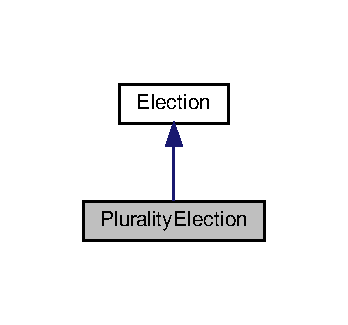
\includegraphics[width=167pt]{classPluralityElection__inherit__graph}
\end{center}
\end{figure}


Collaboration diagram for Plurality\+Election\+:\nopagebreak
\begin{figure}[H]
\begin{center}
\leavevmode
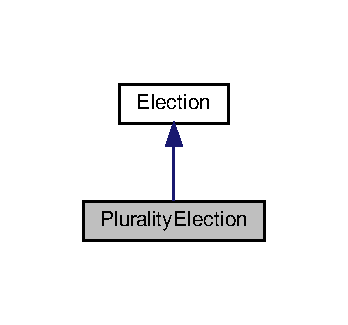
\includegraphics[width=167pt]{classPluralityElection__coll__graph}
\end{center}
\end{figure}
\subsection*{Public Member Functions}
\begin{DoxyCompactItemize}
\item 
\hyperlink{classPluralityElection_a03dd61a9d6738ec26e80d10acb02df7d}{Plurality\+Election} (std\+::string type, int seats, std\+::vector$<$ \hyperlink{classCandidate}{Candidate} $\ast$$>$ cands, std\+::vector$<$ \hyperlink{classBallot}{Ballot} $\ast$$>$ bals)
\item 
void \hyperlink{classPluralityElection_a9517806e8ba40496c49013acc7ad9ca5}{run\+Algorithm} () override
\item 
std\+::string \hyperlink{classPluralityElection_a60f88a34588ca87678b0f5367adf1a55}{get\+Results} () override
\end{DoxyCompactItemize}
\subsection*{Additional Inherited Members}


\subsection{Detailed Description}
The \hyperlink{classPluralityElection}{Plurality\+Election} class is a child class of the abstract \hyperlink{classElection}{Election} class that provides the necessary functionality to represent a Plurality election. 

\subsection{Constructor \& Destructor Documentation}
\mbox{\Hypertarget{classPluralityElection_a03dd61a9d6738ec26e80d10acb02df7d}\label{classPluralityElection_a03dd61a9d6738ec26e80d10acb02df7d}} 
\index{Plurality\+Election@{Plurality\+Election}!Plurality\+Election@{Plurality\+Election}}
\index{Plurality\+Election@{Plurality\+Election}!Plurality\+Election@{Plurality\+Election}}
\subsubsection{\texorpdfstring{Plurality\+Election()}{PluralityElection()}}
{\footnotesize\ttfamily Plurality\+Election\+::\+Plurality\+Election (\begin{DoxyParamCaption}\item[{std\+::string}]{type,  }\item[{int}]{seats,  }\item[{std\+::vector$<$ \hyperlink{classCandidate}{Candidate} $\ast$$>$}]{cands,  }\item[{std\+::vector$<$ \hyperlink{classBallot}{Ballot} $\ast$$>$}]{bals }\end{DoxyParamCaption})}

The constructor for the \hyperlink{classPluralityElection}{Plurality\+Election} class utilizes the constructor of the \hyperlink{classElection}{Election} class to set the type, number of seats, the Candidates in the election, and the Ballots in the election. 
\begin{DoxyParams}{Parameters}
{\em type} & a string that indicates the election type \\
\hline
{\em seats} & an int that indicates the number of seats in the election \\
\hline
{\em cands} & a vector of Candidates who are up for election \\
\hline
{\em bals} & a vector of Ballots that were cast in the election \\
\hline
\end{DoxyParams}
\begin{DoxyAuthor}{Author}
Brendan Ritchie (ritch167) 
\end{DoxyAuthor}


\subsection{Member Function Documentation}
\mbox{\Hypertarget{classPluralityElection_a60f88a34588ca87678b0f5367adf1a55}\label{classPluralityElection_a60f88a34588ca87678b0f5367adf1a55}} 
\index{Plurality\+Election@{Plurality\+Election}!get\+Results@{get\+Results}}
\index{get\+Results@{get\+Results}!Plurality\+Election@{Plurality\+Election}}
\subsubsection{\texorpdfstring{get\+Results()}{getResults()}}
{\footnotesize\ttfamily std\+::string Plurality\+Election\+::get\+Results (\begin{DoxyParamCaption}{ }\end{DoxyParamCaption})\hspace{0.3cm}{\ttfamily [override]}, {\ttfamily [virtual]}}

This method gets the result of running the plurality algorithm. It returns a string variable that contains the results of the plurality election, as well as the Candidates and their vote percentage. Also, the string contains who won and who lost. \begin{DoxyAuthor}{Author}
Yiwen Xu (xu000515) 
\end{DoxyAuthor}


Implements \hyperlink{classElection_a6a6f4f301db86628b8d962281a19bf74}{Election}.

\mbox{\Hypertarget{classPluralityElection_a9517806e8ba40496c49013acc7ad9ca5}\label{classPluralityElection_a9517806e8ba40496c49013acc7ad9ca5}} 
\index{Plurality\+Election@{Plurality\+Election}!run\+Algorithm@{run\+Algorithm}}
\index{run\+Algorithm@{run\+Algorithm}!Plurality\+Election@{Plurality\+Election}}
\subsubsection{\texorpdfstring{run\+Algorithm()}{runAlgorithm()}}
{\footnotesize\ttfamily void Plurality\+Election\+::run\+Algorithm (\begin{DoxyParamCaption}{ }\end{DoxyParamCaption})\hspace{0.3cm}{\ttfamily [override]}, {\ttfamily [virtual]}}

This method is responsible for running the election based on the plurality algorithm. \begin{DoxyAuthor}{Author}
Yiwen Xu (xu000515) 
\end{DoxyAuthor}


Implements \hyperlink{classElection_a059659576ebb0416ecd8005f684461d6}{Election}.



The documentation for this class was generated from the following file\+:\begin{DoxyCompactItemize}
\item 
/home/ritch167/csci5801/repo-\/\+Team4/\+Project1/src/plurality\+\_\+election.\+h\end{DoxyCompactItemize}

\hypertarget{classSTVElection}{}\section{S\+T\+V\+Election Class Reference}
\label{classSTVElection}\index{S\+T\+V\+Election@{S\+T\+V\+Election}}


The \hyperlink{classSTVElection}{S\+T\+V\+Election} class is a child class of the abstract \hyperlink{classElection}{Election} class that provides the necessary functionality to represent a Single-\/\+Transferrable Vote (ranked choice) election using the Droop algorithm. On top of all of the properties of the \hyperlink{classElection}{Election} class, the \hyperlink{classSTVElection}{S\+T\+V\+Election} class also has a value for the Droop quota, a value indicating whether to turn the \hyperlink{classBallot}{Ballot} shuffle on/off, and a vector that stores the order of the shuffled \hyperlink{classBallot}{Ballot} objects for the election.  




{\ttfamily \#include $<$stv\+\_\+election.\+h$>$}



Inheritance diagram for S\+T\+V\+Election\+:\nopagebreak
\begin{figure}[H]
\begin{center}
\leavevmode
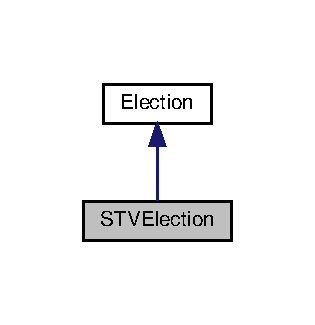
\includegraphics[width=151pt]{classSTVElection__inherit__graph}
\end{center}
\end{figure}


Collaboration diagram for S\+T\+V\+Election\+:\nopagebreak
\begin{figure}[H]
\begin{center}
\leavevmode
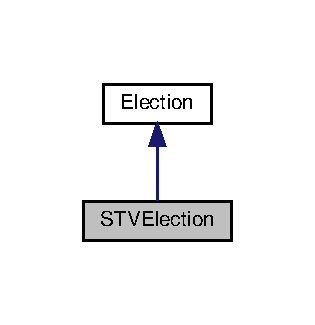
\includegraphics[width=151pt]{classSTVElection__coll__graph}
\end{center}
\end{figure}
\subsection*{Public Member Functions}
\begin{DoxyCompactItemize}
\item 
\hyperlink{classSTVElection_a7869d492ef2d932bd9439516f4252b75}{S\+T\+V\+Election} (std\+::string type, int seats, std\+::vector$<$ \hyperlink{classCandidate}{Candidate} $\ast$$>$ cands, std\+::vector$<$ \hyperlink{classBallot}{Ballot} $\ast$$>$ bals, bool shuffle)
\item 
void \hyperlink{classSTVElection_ac4e0339e3cb97add1a22c9af7233df17}{run\+Algorithm} () override
\item 
int \hyperlink{classSTVElection_a0f8e2dea0af2ecea795a79c6e0e63fe2}{get\+Droop} ()
\item 
bool \hyperlink{classSTVElection_aa8597739fd9823bbe8ea5a7fdb741f53}{get\+Shuffle\+Status} ()
\item 
std\+::vector$<$ int $>$ \hyperlink{classSTVElection_a89e835eb11707dcba9f22a84c1d532f1}{get\+Shuffled\+Ballots} ()
\item 
std\+::string \hyperlink{classSTVElection_ae7efa73091c87add327d71ff5f943c3c}{get\+Results} () override
\end{DoxyCompactItemize}
\subsection*{Additional Inherited Members}


\subsection{Detailed Description}
The \hyperlink{classSTVElection}{S\+T\+V\+Election} class is a child class of the abstract \hyperlink{classElection}{Election} class that provides the necessary functionality to represent a Single-\/\+Transferrable Vote (ranked choice) election using the Droop algorithm. On top of all of the properties of the \hyperlink{classElection}{Election} class, the \hyperlink{classSTVElection}{S\+T\+V\+Election} class also has a value for the Droop quota, a value indicating whether to turn the \hyperlink{classBallot}{Ballot} shuffle on/off, and a vector that stores the order of the shuffled \hyperlink{classBallot}{Ballot} objects for the election. 

\subsection{Constructor \& Destructor Documentation}
\mbox{\Hypertarget{classSTVElection_a7869d492ef2d932bd9439516f4252b75}\label{classSTVElection_a7869d492ef2d932bd9439516f4252b75}} 
\index{S\+T\+V\+Election@{S\+T\+V\+Election}!S\+T\+V\+Election@{S\+T\+V\+Election}}
\index{S\+T\+V\+Election@{S\+T\+V\+Election}!S\+T\+V\+Election@{S\+T\+V\+Election}}
\subsubsection{\texorpdfstring{S\+T\+V\+Election()}{STVElection()}}
{\footnotesize\ttfamily S\+T\+V\+Election\+::\+S\+T\+V\+Election (\begin{DoxyParamCaption}\item[{std\+::string}]{type,  }\item[{int}]{seats,  }\item[{std\+::vector$<$ \hyperlink{classCandidate}{Candidate} $\ast$$>$}]{cands,  }\item[{std\+::vector$<$ \hyperlink{classBallot}{Ballot} $\ast$$>$}]{bals,  }\item[{bool}]{shuffle }\end{DoxyParamCaption})}

The constructor for the \hyperlink{classSTVElection}{S\+T\+V\+Election} class utilizes the constructor of the \hyperlink{classElection}{Election} class to set the type, number of seats, the Candidates in the election, and the Ballots in the election. It the sets the shuffle status of the \hyperlink{classSTVElection}{S\+T\+V\+Election} to the value in shuffle. It also calculates the Droop quota here and defaults the vector that stores the order of the shuffled \hyperlink{classBallot}{Ballot} objects for the election to hold the ints 0 to the number of Ballotsin the election. 
\begin{DoxyParams}{Parameters}
{\em type} & a string that indicates the election type \\
\hline
{\em seats} & an int that indicates the number of seats in the election \\
\hline
{\em cands} & a vector of Candidates who are up for election \\
\hline
{\em bals} & a vector of Ballots that were cast in the election \\
\hline
{\em shuffle} & a boolean that indicates whether to turn the \hyperlink{classBallot}{Ballot} shuffle on/off \\
\hline
\end{DoxyParams}
\begin{DoxyAuthor}{Author}
Brendan Ritchie (ritch167) 
\end{DoxyAuthor}


\subsection{Member Function Documentation}
\mbox{\Hypertarget{classSTVElection_a0f8e2dea0af2ecea795a79c6e0e63fe2}\label{classSTVElection_a0f8e2dea0af2ecea795a79c6e0e63fe2}} 
\index{S\+T\+V\+Election@{S\+T\+V\+Election}!get\+Droop@{get\+Droop}}
\index{get\+Droop@{get\+Droop}!S\+T\+V\+Election@{S\+T\+V\+Election}}
\subsubsection{\texorpdfstring{get\+Droop()}{getDroop()}}
{\footnotesize\ttfamily int S\+T\+V\+Election\+::get\+Droop (\begin{DoxyParamCaption}{ }\end{DoxyParamCaption})}

This method returns the droop quota of the \hyperlink{classSTVElection}{S\+T\+V\+Election} object \begin{DoxyAuthor}{Author}
Brendan Ritchie (ritch167) 
\end{DoxyAuthor}
\mbox{\Hypertarget{classSTVElection_ae7efa73091c87add327d71ff5f943c3c}\label{classSTVElection_ae7efa73091c87add327d71ff5f943c3c}} 
\index{S\+T\+V\+Election@{S\+T\+V\+Election}!get\+Results@{get\+Results}}
\index{get\+Results@{get\+Results}!S\+T\+V\+Election@{S\+T\+V\+Election}}
\subsubsection{\texorpdfstring{get\+Results()}{getResults()}}
{\footnotesize\ttfamily std\+::string S\+T\+V\+Election\+::get\+Results (\begin{DoxyParamCaption}{ }\end{DoxyParamCaption})\hspace{0.3cm}{\ttfamily [override]}, {\ttfamily [virtual]}}

This method returns the result of an election with S\+TV algorithm \begin{DoxyAuthor}{Author}
Yifan Zhang (zhan4372) 
\end{DoxyAuthor}


Implements \hyperlink{classElection_a6a6f4f301db86628b8d962281a19bf74}{Election}.

\mbox{\Hypertarget{classSTVElection_a89e835eb11707dcba9f22a84c1d532f1}\label{classSTVElection_a89e835eb11707dcba9f22a84c1d532f1}} 
\index{S\+T\+V\+Election@{S\+T\+V\+Election}!get\+Shuffled\+Ballots@{get\+Shuffled\+Ballots}}
\index{get\+Shuffled\+Ballots@{get\+Shuffled\+Ballots}!S\+T\+V\+Election@{S\+T\+V\+Election}}
\subsubsection{\texorpdfstring{get\+Shuffled\+Ballots()}{getShuffledBallots()}}
{\footnotesize\ttfamily std\+::vector$<$int$>$ S\+T\+V\+Election\+::get\+Shuffled\+Ballots (\begin{DoxyParamCaption}{ }\end{DoxyParamCaption})}

This method returns the vector of shullfed index of ballots of the \hyperlink{classSTVElection}{S\+T\+V\+Election} object \begin{DoxyAuthor}{Author}
Brendan Ritchie (ritch167) 
\end{DoxyAuthor}
\mbox{\Hypertarget{classSTVElection_aa8597739fd9823bbe8ea5a7fdb741f53}\label{classSTVElection_aa8597739fd9823bbe8ea5a7fdb741f53}} 
\index{S\+T\+V\+Election@{S\+T\+V\+Election}!get\+Shuffle\+Status@{get\+Shuffle\+Status}}
\index{get\+Shuffle\+Status@{get\+Shuffle\+Status}!S\+T\+V\+Election@{S\+T\+V\+Election}}
\subsubsection{\texorpdfstring{get\+Shuffle\+Status()}{getShuffleStatus()}}
{\footnotesize\ttfamily bool S\+T\+V\+Election\+::get\+Shuffle\+Status (\begin{DoxyParamCaption}{ }\end{DoxyParamCaption})}

This method returns the status of the shullfle option of the \hyperlink{classSTVElection}{S\+T\+V\+Election} object \begin{DoxyAuthor}{Author}
Brendan Ritchie (ritch167) 
\end{DoxyAuthor}
\mbox{\Hypertarget{classSTVElection_ac4e0339e3cb97add1a22c9af7233df17}\label{classSTVElection_ac4e0339e3cb97add1a22c9af7233df17}} 
\index{S\+T\+V\+Election@{S\+T\+V\+Election}!run\+Algorithm@{run\+Algorithm}}
\index{run\+Algorithm@{run\+Algorithm}!S\+T\+V\+Election@{S\+T\+V\+Election}}
\subsubsection{\texorpdfstring{run\+Algorithm()}{runAlgorithm()}}
{\footnotesize\ttfamily void S\+T\+V\+Election\+::run\+Algorithm (\begin{DoxyParamCaption}{ }\end{DoxyParamCaption})\hspace{0.3cm}{\ttfamily [override]}, {\ttfamily [virtual]}}

This is the primary function which is used to run the algorithm to determine winners and losers for an S\+TV \hyperlink{classElection}{Election}. It shuffles the ballots if necessary, initially distributes them to candidates, and then relies on the redistribute() function to handle ballot redistribution from there on out. It also makes use of the \hyperlink{classElection_abd52b6c894a9f2a0a0a104e9f290f9a7}{write\+To\+Audit\+File()} to write the necessary information for election auditing to the designated text file. \begin{DoxyAuthor}{Author}
Brendan Ritchie (ritch167) 
\end{DoxyAuthor}


Implements \hyperlink{classElection_a059659576ebb0416ecd8005f684461d6}{Election}.



The documentation for this class was generated from the following file\+:\begin{DoxyCompactItemize}
\item 
/home/ritch167/csci5801/repo-\/\+Team4/\+Project1/src/stv\+\_\+election.\+h\end{DoxyCompactItemize}

\hypertarget{classVotingApp}{}\section{Voting\+App Class Reference}
\label{classVotingApp}\index{Voting\+App@{Voting\+App}}


The \hyperlink{classVotingApp}{Voting\+App} class provides the necessary functionality to run the user interface for the application. It handles all interactions with the user in the interface and initiates the process of running an election after being given all the necessary information by the user. It also provides the necessary functionality to run in a test mode for debugging purposes.  




{\ttfamily \#include $<$voting\+\_\+app.\+h$>$}

\subsection*{Public Member Functions}
\begin{DoxyCompactItemize}
\item 
\hyperlink{classVotingApp_a23dbc45972a7246f7f4449c831af6c75}{Voting\+App} (bool test\+\_\+mode)
\item 
void \hyperlink{classVotingApp_a9d62b11e6082588a0b01752f838e0611}{run} ()
\end{DoxyCompactItemize}


\subsection{Detailed Description}
The \hyperlink{classVotingApp}{Voting\+App} class provides the necessary functionality to run the user interface for the application. It handles all interactions with the user in the interface and initiates the process of running an election after being given all the necessary information by the user. It also provides the necessary functionality to run in a test mode for debugging purposes. 

\subsection{Constructor \& Destructor Documentation}
\mbox{\Hypertarget{classVotingApp_a23dbc45972a7246f7f4449c831af6c75}\label{classVotingApp_a23dbc45972a7246f7f4449c831af6c75}} 
\index{Voting\+App@{Voting\+App}!Voting\+App@{Voting\+App}}
\index{Voting\+App@{Voting\+App}!Voting\+App@{Voting\+App}}
\subsubsection{\texorpdfstring{Voting\+App()}{VotingApp()}}
{\footnotesize\ttfamily Voting\+App\+::\+Voting\+App (\begin{DoxyParamCaption}\item[{bool}]{test\+\_\+mode }\end{DoxyParamCaption})}

The constructor for the \hyperlink{classVotingApp}{Voting\+App} class sets test mode status of the object. It defaults the \hyperlink{classElection}{Election} member variable to N\+U\+LL. 
\begin{DoxyParams}{Parameters}
{\em test\+\_\+mode} & a boolean that indicates whether the application is running in test mode or not \\
\hline
\end{DoxyParams}
\begin{DoxyAuthor}{Author}
Brendan Ritchie (ritch167) 
\end{DoxyAuthor}


\subsection{Member Function Documentation}
\mbox{\Hypertarget{classVotingApp_a9d62b11e6082588a0b01752f838e0611}\label{classVotingApp_a9d62b11e6082588a0b01752f838e0611}} 
\index{Voting\+App@{Voting\+App}!run@{run}}
\index{run@{run}!Voting\+App@{Voting\+App}}
\subsubsection{\texorpdfstring{run()}{run()}}
{\footnotesize\ttfamily void Voting\+App\+::run (\begin{DoxyParamCaption}{ }\end{DoxyParamCaption})}

This is the run method for the voting system. No inputs and returns nothing. \begin{DoxyAuthor}{Author}
Sara Nelson (nels8907) 
\end{DoxyAuthor}


The documentation for this class was generated from the following file\+:\begin{DoxyCompactItemize}
\item 
/home/ritch167/csci5801/repo-\/\+Team4/\+Project1/src/voting\+\_\+app.\+h\end{DoxyCompactItemize}

%--- End generated contents ---

% Index
\backmatter
\newpage
\phantomsection
\clearemptydoublepage
\addcontentsline{toc}{chapter}{Index}
\printindex

\end{document}
